% !TeX program = xelatex
\ifdefined\BookMaster\else
\documentclass[11pt,oneside]{article}
% !TeX program = xelatex
\usepackage[b5paper,left=22mm,right=22mm,top=20mm,bottom=22mm,footskip=11mm]{geometry}
\usepackage{fontspec}
\setmainfont{TeX Gyre Termes}
\setsansfont{TeX Gyre Heros}
\usepackage{amsmath,amssymb,mathtools,amsthm}
\renewcommand{\cdots}{\mathinner{\cdotp\cdotp\cdotp}}
\usepackage{graphicx,adjustbox,array,booktabs,longtable,multirow,enumitem,changepage,needspace}
\usepackage[table]{xcolor}
\usepackage{fancyhdr}
\raggedbottom
\interfootnotelinepenalty=10000
\newcommand{\BookFootnote}[2]{\begingroup\renewcommand{\thefootnote}{\fnsymbol{footnote}}\footnote[#1]{#2}\endgroup}
\newcommand{\BookFootnoteMark}[1]{\begingroup\renewcommand{\thefootnote}{\fnsymbol{footnote}}\footnotemark[#1]\endgroup}
\newcommand{\BookFootnoteText}[2]{\begingroup\renewcommand{\thefootnote}{\fnsymbol{footnote}}\footnotetext[#1]{#2}\endgroup}
\newenvironment{BookFloat}[1]{\par\addvspace{.6\baselineskip}\noindent\def\BookFloatID{#1}\begin{minipage}{\linewidth}\phantomsection\label{bookfloat:#1:start}}{\phantomsection\label{bookfloat:\BookFloatID:end}\end{minipage}\par\addvspace{.6\baselineskip}}

\usepackage[unicode,hidelinks]{hyperref}
\pagestyle{fancy}
\fancyhf{}
\newcommand{\BookFooter}{}
\fancyfoot[L]{\parbox[b]{\dimexpr\textwidth-15mm}{\footnotesize\BookFooter}}
\fancyfoot[R]{\footnotesize\thepage}
\renewcommand{\headrulewidth}{0pt}
\renewcommand{\footrulewidth}{0pt}
\setlength{\parindent}{0pt}
\setlength{\parskip}{0.2em}
\setlength{\emergencystretch}{3em}
\setlist{nosep,leftmargin=1.7em,labelsep=.65em}
\newif\ifBookNarrative
\BookNarrativetrue
\newenvironment{BookBody}{\setlength{\parindent}{0pt}}{}
\newcommand{\BookStatement}[1]{\par\addvspace{.6\baselineskip}\noindent #1\enspace\ignorespaces}
\newcommand{\BookLabel}[1]{\par\addvspace{.6\baselineskip}\needspace{3\baselineskip}\noindent\textbf{#1}\quad\ignorespaces}
\newcommand{\BookHeading}[1]{\par\addvspace{\baselineskip}\needspace{4\baselineskip}\noindent{\large\bfseries #1}\par\medskip}
\newcommand{\BookSubheading}[1]{\par\addvspace{.7\baselineskip}\needspace{3\baselineskip}\noindent{\bfseries #1}\par\smallskip}
\newcommand{\BookTextHeading}[1]{\par\addvspace{.7\baselineskip}\needspace{3\baselineskip}\noindent #1\par\smallskip}
\newcommand{\BookSectionTitle}[2]{\par\addvspace{1.2\baselineskip}\needspace{5\baselineskip}\noindent\colorbox{gray!25}{\sffamily\bfseries\small SECTION #1}\quad{\large\bfseries #2}\par\medskip}
\newcommand{\BookExerciseTitle}[1]{\par\addvspace{\baselineskip}\needspace{4\baselineskip}\noindent{\color{gray}\rule{1.5mm}{1.5mm}}\enspace{\large\bfseries Exercises #1}\par\medskip}
\newcommand{\BookBullet}[1]{\begin{list}{\textbullet}{\setlength{\leftmargin}{1.7em}\setlength{\labelwidth}{1em}\setlength{\labelsep}{.7em}\setlength{\topsep}{0pt}\setlength{\parsep}{0pt}\setlength{\itemsep}{0pt}}\item #1\end{list}}
\newcommand{\BookExercise}[2]{\begin{list}{\textbf{#1}}{\setlength{\leftmargin}{2.2em}\setlength{\labelwidth}{1.5em}\setlength{\labelsep}{.7em}\setlength{\topsep}{.15em}\setlength{\parsep}{0pt}\setlength{\itemsep}{0pt}}\item #2\end{list}}
\newcommand{\BookEnd}[1]{\unskip\nobreak\hfill\ensuremath{#1}}
\newcommand{\BookSource}[2]{\phantomsection\label{sourcepage:#1}} % Source-page anchors, retained through reflow.
\usepackage{multicol}
\usepackage{tikz}
\newcommand{\BookPartEntry}[2]{\par\noindent\makebox[17mm][l]{\bfseries Section #1}#2\par}
\newcommand{\BookPartTitle}[3]{\par\bigskip\noindent\begin{tikzpicture}\node[anchor=north west,inner sep=0pt,outer sep=0pt] (bookpart) at (0,0) {\begin{minipage}{\dimexpr\linewidth-.5pt}\hspace*{26mm}\begin{minipage}[t]{\dimexpr\linewidth-26mm}\begin{adjustbox}{max width=\linewidth}{\fontsize{20}{24}\selectfont\bfseries #2}\end{adjustbox}\par\vspace{6mm}\hrule\vspace{6mm}{\sffamily\footnotesize\setlength{\parskip}{.3em}#3}\vspace{3mm}\end{minipage}\end{minipage}};\path[shade,top color=gray!60,bottom color=white] (0,0) rectangle ([xshift=24mm]bookpart.south west);\node[anchor=north,font=\sffamily\bfseries\small] at (12mm,-2mm) {PART};\node[anchor=north,font=\sffamily\bfseries\Huge] at (12mm,-7mm) {#1};\end{tikzpicture}\par\bigskip}
\newsavebox{\BookMathBox}
\makeatletter
\newcommand{\BookInline}[1]{\leavevmode\hskip0pt\relax\begingroup\in@{\begin}{#1}\ifin@\sbox{\BookMathBox}{\(#1\)}\ifdim\wd\BookMathBox>\dimexpr\linewidth-1em\relax\resizebox{\dimexpr\linewidth-1em\relax}{!}{\usebox{\BookMathBox}}\else\(#1\)\fi\else\in@{\left}{#1}\ifin@\sbox{\BookMathBox}{\(#1\)}\ifdim\wd\BookMathBox>\dimexpr\linewidth-1em\relax\resizebox{\dimexpr\linewidth-1em\relax}{!}{\usebox{\BookMathBox}}\else\(#1\)\fi\else\(#1\)\fi\fi\endgroup\hskip0pt\relax}
\makeatother
\DeclareMathOperator{\Aut}{Aut}
\DeclareMathOperator{\End}{End}
\DeclareMathOperator{\Hom}{Hom}
\DeclareMathOperator{\GF}{GF}
\DeclareMathOperator{\irr}{irr}
\DeclareMathOperator{\lt}{lt}
\DeclareMathOperator{\lp}{lp}
\providecommand{\textcircled}[1]{\textnormal{(#1)}}

\begin{document}
\fi
\renewcommand{\BookFooter}{Section 40 Algebraic Extensions}
\pdfbookmark[0]{Section 40 Algebraic Extensions}{40_algebraic_extensions}
\ifdefined\BookMaster\else\setcounter{page}{319}\fi
% Source PDF page 336; original printed page 319
\BookSource{336}{319}
\BookNarrativetrue

\begin{BookBody}

\BookSectionTitle{40}{Algebraic Extensions}

\BookTextHeading{\textbf{Finite Extensions}  }

\noindent In Corollary 39.23 we saw that if \BookInline{E} is an extension field of a field \BookInline{F} and \BookInline{\alpha \in E} is algebraic over \BookInline{F,\allowbreak } then every element of \BookInline{F(\alpha )} is algebraic over \BookInline{F.} In studying zeros of polynomials in \BookInline{F[x],\allowbreak } we shall be interested almost exclusively in extensions of \BookInline{F} containing only elements algebraic over \BookInline{F.}

\BookLabel{40.1 Definition} An extension field \BookInline{E} of a field \BookInline{F} is an\textbf{ algebraic extension of} \BookInline{F} if every element in \BookInline{E} is algebraic over \BookInline{F.}\BookEnd{\blacksquare}

\BookLabel{40.2 Definition} If an extension field \BookInline{E} of a field \BookInline{F} is of finite dimension \BookInline{n} as a vector space over \BookInline{F,\allowbreak } then \BookInline{E} is a\textbf{ finite extension of degree} \BookInline{n} \textbf{over} \BookInline{F.} We shall let \BookInline{[E:F]} be the degree \BookInline{n} of \BookInline{E} over \BookInline{F.}\BookEnd{\blacksquare}

\end{BookBody}

% Source PDF page 337; original printed page 320
\BookSource{337}{320}
\BookNarrativetrue

\begin{BookBody}

To say that a field \BookInline{E} is a finite extension of a field \BookInline{F} does\textit{ not} mean that \BookInline{E} is a finite field. It just asserts that \BookInline{E} is a finite-dimensional vector space over \BookInline{F,\allowbreak } that is, that \BookInline{[E:F]} is finite.

We shall often use the fact that if \BookInline{E} is a finite extension of \BookInline{F,\allowbreak } then\BookInline{,\allowbreak [E:F]= 1} if and only if \BookInline{E= F.} We need only observe that by Theorem \BookInline{33.18,\allowbreak \{1\}} can always be enlarged to a basis for \BookInline{E} over \BookInline{F.} Thus \BookInline{[E:F]= 1} if and only if \BookInline{E= F(1)= F.}

We show that a finite extension \BookInline{E} of a field \BookInline{F} must be an algebraic extension of \BookInline{F.}

\BookLabel{40.3 Theorem} A finite extension field \BookInline{E} of a field \BookInline{F} is an algebraic extension of \BookInline{F.}

\BookLabel{\textit{Proof}} We must show that for \BookInline{\alpha \in E,\allowbreak \alpha } is algebraic over \BookInline{F.} By Theorem 33.18 if \BookInline{[E:F]= n,\allowbreak } then \BookInline{n}

\begin{center}\begin{adjustbox}{max width=\linewidth}\BookInline{\displaystyle 1,\allowbreak \alpha ,\allowbreak \cdots ,\allowbreak \alpha}\end{adjustbox}\end{center}

\noindent cannot be linearly independent elements, so there exist \BookInline{a_{i}\in F} such that

\begin{center}\begin{adjustbox}{max width=\linewidth}\BookInline{\displaystyle a_{n}\alpha ^{n}+ \cdots + a_{1}\alpha + a_{0}= 0,\allowbreak }\end{adjustbox}\end{center}

\noindent and not all \BookInline{a_{i}= 0.} Then \BookInline{f(x)= a_{n}x^{n}+ \cdots + a_{1}x+ a_{0}} is a nonzero polynomial in \BookInline{F[x],\allowbreak } and \BookInline{f(\alpha )= 0.} Therefore\BookInline{,\allowbreak \alpha } is algebraic over \BookInline{F.}\BookEnd{\blacklozenge}

We cannot overemphasize the importance of our next theorem. It plays a role in field theory analogous to the role of the theorem of Lagrange in group theory. While its proof follows easily from our brief work with vector spaces, it is a tool of incredible power. An elegant application of it in the section that follows shows the impossibility of performing certain geometric constructions with a straightedge and a compass.\textit{ Never} \textit{underestimate} \BookInline{a} \textit{theorem that counts something.}

\BookLabel{40.4 Theorem} If \BookInline{E} is a finite extension field of a field \BookInline{F,\allowbreak } and \BookInline{K} is a finite extension field of \BookInline{E,\allowbreak } then \BookInline{K} is a finite extension of \BookInline{F,\allowbreak } and

\begin{center}\begin{adjustbox}{max width=\linewidth}\BookInline{\displaystyle [K:F]= [K:E][E:F].}\end{adjustbox}\end{center}

\BookLabel{\textit{Proof}} Let \BookInline{\{\alpha _{i}\mid i= 1,\allowbreak \cdots,\allowbreak n\}} be a basis for \BookInline{E} as a vector space over \BookInline{F,\allowbreak } and let the set \BookInline{\{\beta _{j}\mid j= 1,\allowbreak \cdots,\allowbreak m\}} be a basis for \BookInline{K} as a vector space over \BookInline{E.} The theorem will be proved if we can show that the \BookInline{mn} elements \BookInline{\alpha _{i}\beta _{j}} form a basis for \BookInline{K,\allowbreak } viewed as a vector space over \BookInline{F.(}See Fig. 40.5.)

Let \BookInline{\gamma } be any element of \BookInline{K.} Since the \BookInline{\beta _{j}} form a basis for \BookInline{K} over \BookInline{E,\allowbreak } we have

\begin{center}\begin{adjustbox}{max width=\linewidth}\BookInline{\displaystyle \gamma = \sum _{j= 1}^{m}b_{j}\beta _{j}}\end{adjustbox}\end{center}

\noindent for some \BookInline{b_{j}\in E.} Since the \BookInline{\alpha _{i}} form a basis for \BookInline{E} over \BookInline{F,\allowbreak } we have

\begin{center}\begin{adjustbox}{max width=\linewidth}\BookInline{\displaystyle b_{j}= \sum _{i= 1}^{n}a_{ij}\alpha _{i}}\end{adjustbox}\end{center}

\noindent for some \BookInline{a_{ij}\in F.} Then

\begin{center}\begin{adjustbox}{max width=\linewidth}\BookInline{\displaystyle \gamma = \sum _{j= 1}^{m}\Big(\sum _{i= 1}^{n}a_{ij}\alpha _{i}\Big)\beta _{j}= \sum _{i,\allowbreak j}a_{ij}(\alpha _{i}\beta _{j}),\allowbreak }\end{adjustbox}\end{center}

\noindent so the \BookInline{mn} vectors \BookInline{\alpha _{i}\beta _{j}} span \BookInline{K} over \BookInline{F.}

It remains for us to show that the \BookInline{mn} elements \BookInline{\alpha _{i}\beta _{j}} are independent over \BookInline{F.} Suppose that \BookInline{\Sigma _{i,\allowbreak j}c_{ij}(\alpha _{i}\beta _{j})= 0,\allowbreak } with \BookInline{c_{ij}\in F.} Then

\begin{center}\begin{adjustbox}{max width=\linewidth}\BookInline{\displaystyle \sum _{j= 1}^{m}\Big(\sum _{i= 1}^{n}c_{ij}\alpha _{i}\Big)\beta _{j}= 0,\allowbreak }\end{adjustbox}\end{center}

\noindent and \BookInline{(\Sigma }\textit{in}\BookInline{= 1cij\alpha i)\in E.} Since the elements \BookInline{\beta _{j}} are independent over \BookInline{E,\allowbreak } we must have

\end{BookBody}

% Source PDF page 338; original printed page 321
\BookSource{338}{321}
\BookNarrativetrue

\begin{BookBody}

\begin{BookFloat}{40_algebraic_extensions-p338-0}
\begin{center}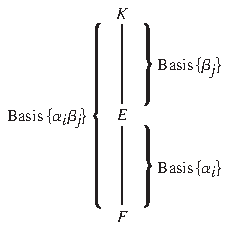
\includegraphics[width=0.310\linewidth,height=.8\textheight,keepaspectratio]{assets/p338_03.pdf}\end{center}
\begin{center}\small\textbf{40.5 Figure}\end{center}
\end{BookFloat}

\begin{center}\begin{adjustbox}{max width=\linewidth}\BookInline{\displaystyle \sum _{i= 1}^{n}c_{ij}\alpha _{i}= 0}\end{adjustbox}\end{center}

\noindent for all \BookInline{j.} But now the \BookInline{\alpha _{i}} are independent over \BookInline{F,\allowbreak } so \BookInline{\sum _{i= 1}^{n}c_{ij}\alpha _{i}= 0} implies that \BookInline{c_{ij}= 0} for all \BookInline{i} and \BookInline{j.} Thus the \BookInline{\alpha _{i}\beta _{j}} not only span \BookInline{K} over \BookInline{F} but also are independent over \BookInline{F.} Thus they form a basis for \BookInline{K} over \BookInline{F.}\BookEnd{\blacklozenge}

Note that we proved this theorem by actually exhibiting a basis. It is worth remembering that if \BookInline{\{\alpha _{i}\mid i= 1,\allowbreak \cdots,\allowbreak n\}} is a basis for \BookInline{E} over \BookInline{F} and \BookInline{\{\beta _{j}\mid j= 1,\allowbreak \cdots,\allowbreak m\}} is a basis for \BookInline{K} over \BookInline{E,\allowbreak } for fields \BookInline{F\leq E\leq K,\allowbreak } then the set \BookInline{\{\alpha _{i}\beta _{j}\}} of \BookInline{mn} products is a basis for \BookInline{K} over \BookInline{F.} Figure 40.5 gives a diagram for this situation. We shall illustrate this further in a moment.

\BookLabel{40.6 Corollary} If \BookInline{F_{i}} is a field for \BookInline{i= 1,\allowbreak \cdots,\allowbreak r} and \BookInline{F_{i+ 1}} is a finite extension of \BookInline{F_{i},\allowbreak } then \BookInline{F_{r}} is a finite extension of \BookInline{F_{1},\allowbreak } and

\begin{center}\begin{adjustbox}{max width=\linewidth}\BookInline{\displaystyle [F_{r}:F_{1}]= [F_{r}:F_{r- 1}][F_{r- 1}:F_{r- 2}]\cdots [F_{2}:F_{1}].}\end{adjustbox}\end{center}

\BookLabel{\textit{Proof}} The proof is a straightforward extension of Theorem 40.4 by induction. \BookEnd{\blacklozenge}

\BookLabel{40.7 Corollary} If \BookInline{E} is an extension field of \BookInline{F,\allowbreak \alpha \in E} is algebraic over \BookInline{F,\allowbreak } and \BookInline{\beta \in F(\alpha ),\allowbreak } then deg\BookInline{(\beta,\allowbreak F)} divides deg\BookInline{(\alpha,\allowbreak F).}

\BookLabel{\textit{Proof}} By Corollary 39.23, deg\BookInline{(\alpha,\allowbreak F)= [F(\alpha ):F]} and deg\BookInline{(\beta,\allowbreak F)= [F(\beta ):F].} We have \BookInline{F\leq } \BookInline{F(\beta )\leq F(\alpha ),\allowbreak } so by Corollary \BookInline{40.6[F(\beta ):F]} divides \BookInline{[F(\alpha ):F].}\BookEnd{\blacklozenge}

The following example illustrates a type of argument one often makes using Theorem 40.4 or its corollaries.

\BookLabel{40.8 Example} By Corollary 40.7, there is no element of \BookInline{\mathbb{Q}(\sqrt{2})} that is a zero of \BookInline{x^{3}- 2.} Note that deg\BookInline{(\sqrt{2},\allowbreak \mathbb{Q})= 2,\allowbreak } while a zero of \BookInline{x^{3}- 2} is of degree 3 over \BookInline{\mathbb{Q},\allowbreak } but 3 does not divide 2. \BookEnd{\blacktriangle}

Let \BookInline{E} be an extension field of a field \BookInline{F,\allowbreak } and let \BookInline{\alpha _{1},\allowbreak \alpha _{2}} be elements of \BookInline{E,\allowbreak } not necessarily algebraic over \BookInline{F.} By definition\BookInline{,\allowbreak F(\alpha _{1})} is the smallest extension field of \BookInline{F} in \BookInline{E} that contains \BookInline{\alpha _{1}.} Similarly\BookInline{,\allowbreak (F(\alpha _{1}))(\alpha _{2})} can be characterized as the smallest extension field of \BookInline{F} in \BookInline{E} containing both \BookInline{\alpha _{1}} and \BookInline{\alpha _{2}.} We could equally have started with \BookInline{\alpha _{2},\allowbreak } so \BookInline{(F(\alpha _{1}))(\alpha _{2})= (F(\alpha _{2}))(\alpha _{1}).} We denote this field by \BookInline{F(\alpha _{1},\allowbreak \alpha _{2}).} Similarly, for \BookInline{\alpha _{i}\in E,\allowbreak F(\alpha _{1},\allowbreak \cdots,\allowbreak \alpha _{n})} is the smallest extension field of \BookInline{F} in \BookInline{E} containing all the \BookInline{\alpha _{i}} for \BookInline{i= 1,\allowbreak \cdots,\allowbreak n.} We obtain the field \BookInline{F(\alpha _{1},\allowbreak \cdots,\allowbreak \alpha _{n})} from the field \BookInline{F} by\textbf{ adjoining to} \BookInline{F} \textbf{the} \textbf{elements} \BookInline{\alpha _{i}} in \BookInline{E.} Exercise 51 of Section 22 shows that, analogous to an intersection of subgroups of a group, an intersection of subfields of a field \BookInline{E} is again a subfield of \BookInline{E.} Thus \BookInline{F(\alpha _{1},\allowbreak \cdots,\allowbreak \alpha _{n})} can be characterized as the intersection of all subfields of \BookInline{E} containing \BookInline{F} and all the \BookInline{\alpha _{i}} for \BookInline{i= 1,\allowbreak \cdots,\allowbreak n.}

\end{BookBody}

% Source PDF page 339; original printed page 322
\BookSource{339}{322}
\BookNarrativetrue

\begin{BookBody}

\BookLabel{40.9 Example} Consider \BookInline{\mathbb{Q}(\sqrt{2}).} Corollary 39.23 shows that \BookInline{\{1,\allowbreak \sqrt{2}\}} is a basis for \BookInline{\mathbb{Q}(\sqrt{2})} over \BookInline{\mathbb{Q}.} Using the technique demonstrated in Example 39.10, we can easily discover that \BookInline{\sqrt{2}+ \sqrt{3}} is a zero of \BookInline{x^{4}- 10x^{2}+ 1.} By the method demonstrated in Example 28.15, we can show that this polynomial is irreducible in \BookInline{\mathbb{Q}[x]}. Thus irr \BookInline{( \sqrt{2} + \sqrt{3},\allowbreak \mathbb{Q} ) = x^4 - 10x^2 + 1}, so \BookInline{[ \mathbb { Q } ( { \sqrt { 2 } } + { \sqrt { 3 } } ): \mathbb { Q } ] = 4.} Thus \BookInline{( { \sqrt { 2 } } + { \sqrt { 3 } } ) \not \in \mathbb { Q } ( { \sqrt { 2 } } )}, so \BookInline{{ \sqrt { 3 } } \notin \mathbb { Q } ( { \sqrt { 2 } } )}. Consequently, \BookInline{\{1,\allowbreak \sqrt{3}\}} is a basis for \BookInline{\mathbb{Q}(\sqrt{2},\allowbreak \sqrt{3})= (\mathbb{Q}(\sqrt{2}))(\sqrt{3})} over \BookInline{\mathbb{Q}(\sqrt{2}).} The proof of Theorem 40.4 (see the comment following the theorem) then shows that \BookInline{\{1,\allowbreak \sqrt{2},\allowbreak \sqrt{3},\allowbreak \sqrt{6}\}} is a basis for \BookInline{\mathbb{Q}(\sqrt{2},\allowbreak \sqrt{3})} over \BookInline{\mathbb{Q}.}\BookEnd{\blacktriangle}

\BookLabel{40.10 Example} Let \BookInline{2^{1/3}} be the real cube root of 2 and \BookInline{2^{1/2}} be the positive square root of 2. Then \BookInline{2^{1/2}\notin \mathbb{Q}(2^{1/3})} because deg\BookInline{(2^{1/2},\allowbreak \mathbb{Q})= 2} and 2 is not a divisor of \BookInline{3= } deg\BookInline{(2^{1/3},\allowbreak \mathbb{Q}).} Thus \BookInline{[\mathbb{Q}(2^{1/3},\allowbreak 2^{1/2}):\mathbb{Q}(2^{1/3})]= 2.} Hence \BookInline{\{1,\allowbreak 2^{1/3},\allowbreak 2^{2/3}\}} is a basis for \BookInline{\mathbb{Q}(2^{1/3})} over \BookInline{\mathbb{Q}} and \BookInline{\{1,\allowbreak 2^{1/2}\}} is a basis for \BookInline{\mathbb{Q}(2^{1/3},\allowbreak 2^{1/2})} over \BookInline{\mathbb{Q}(2^{1/3}).} Furthermore, by Theorem 40.4 (see the comment following the theorem),

\begin{center}\begin{adjustbox}{max width=\linewidth}\BookInline{\displaystyle \{1,\allowbreak 2^{1/2},\allowbreak 2^{1/3},\allowbreak 2^{5/6},\allowbreak 2^{2/3},\allowbreak 2^{7/6}\}}\end{adjustbox}\end{center}

\noindent is a basis for \BookInline{\mathbb{Q}(2^{1/2},\allowbreak 2^{1/3})} over \BookInline{\mathbb{Q}.} Because \BookInline{2^{7/6}= 2(2^{1/6}),\allowbreak } we have \BookInline{2^{1/6}\in \mathbb{Q}(2^{1/2},\allowbreak 2^{1/3}).} Now \BookInline{2^{1/6}} is a zero of \BookInline{x^{6}- 2,\allowbreak } which is irreducible over \BookInline{\mathbb{Q},\allowbreak } by Eisenstein’s criterion, with \BookInline{p= 2.} Thus

\begin{center}\begin{adjustbox}{max width=\linewidth}\BookInline{\displaystyle \mathbb{Q}\leq \mathbb{Q}(2^{1/6})\leq \mathbb{Q}(2^{1/2},\allowbreak 2^{1/3})}\end{adjustbox}\end{center}

\noindent and by Theorem 40.4

\begin{center}\begin{adjustbox}{max width=\linewidth}\BookInline{\displaystyle \begin{aligned}6&= [\mathbb{Q}(2^{1/2},\allowbreak 2^{1/3}):\mathbb{Q}]= [\mathbb{Q}(2^{1/2},\allowbreak 2^{1/3}):\mathbb{Q}(2^{1/6})][\mathbb{Q}(2^{1/6}):\mathbb{Q}] \\ &= [\mathbb{Q}(2^{1/2},\allowbreak 2^{1/3}):\mathbb{Q}(2^{1/6})](6).\end{aligned}}\end{adjustbox}\end{center}

\noindent Therefore, we must have

\begin{center}\begin{adjustbox}{max width=\linewidth}\BookInline{\displaystyle [\mathbb{Q}(2^{1/2},\allowbreak 2^{1/3}):\mathbb{Q}(2^{1/6})]= 1,\allowbreak }\end{adjustbox}\end{center}

\noindent so \BookInline{\mathbb{Q}(2^{1/2},\allowbreak 2^{1/3})= \mathbb{Q}(2^{1/6}),\allowbreak } by the comment preceding Theorem 40.3. \BookEnd{\blacktriangle}

Example 40.10 shows that it is possible for an extension \BookInline{F(\alpha _{1},\allowbreak \cdots,\allowbreak \alpha _{n})} of a field \BookInline{F} to be actually a simple extension, even though \BookInline{n>1.}

Let us characterize extensions of \BookInline{F} of the form \BookInline{F(\alpha _{1},\allowbreak \cdots,\allowbreak \alpha _{n})} in the case that all the \BookInline{\alpha _{i}} are algebraic over \BookInline{F.}

\BookLabel{40.11 Theorem} Let \BookInline{E} be an algebraic extension of a field \BookInline{F.} Then there exist a finite number of elements \BookInline{\alpha _{1},\allowbreak \cdots,\allowbreak \alpha _{n}} in \BookInline{E} such that \BookInline{E= F(\alpha _{1},\allowbreak \cdots,\allowbreak \alpha _{n})} if and only if \BookInline{E} is a finite-dimensional vector space over \BookInline{F,\allowbreak } that is, if and only if \BookInline{E} is a finite extension of \BookInline{F.}

\BookLabel{\textit{Proof}} Suppose that \BookInline{E= F(\alpha _{1},\allowbreak \cdots,\allowbreak \alpha _{n}).} Since \BookInline{E} is an algebraic extension of \BookInline{F,\allowbreak } each \BookInline{\alpha _{i}} is algebraic over \BookInline{F,\allowbreak } so each \BookInline{\alpha _{i}} is algebraic over every extension field of \BookInline{F} in \BookInline{E.} Thus \BookInline{F(\alpha _{1})} is algebraic over \BookInline{F,\allowbreak } and in general\BookInline{,\allowbreak F(\alpha _{1},\allowbreak \cdots,\allowbreak \alpha _{j})} is algebraic over \BookInline{F(\alpha _{i},\allowbreak \cdots,\allowbreak \alpha _{j- 1})} for \BookInline{j= 2,\allowbreak \cdots,\allowbreak n.} Corollary 40.6 applied to the sequence of finite extensions

\begin{center}\begin{adjustbox}{max width=\linewidth}\BookInline{\displaystyle F,\allowbreak F(\alpha _{1}),\allowbreak F(\alpha _{1},\allowbreak \alpha _{2}),\allowbreak \cdots ,\allowbreak F(\alpha _{1},\allowbreak \cdots ,\allowbreak \alpha _{n})= E}\end{adjustbox}\end{center}

\noindent then shows that \BookInline{E} is a finite extension of \BookInline{F.}

Conversely, suppose that \BookInline{E} is a finite algebraic extension of \BookInline{F.} If \BookInline{[E:F]= 1,\allowbreak } then \BookInline{E= F(1)= F,\allowbreak } and we are done. If \BookInline{E\neq F,\allowbreak } let \BookInline{\alpha _{1}\in E,\allowbreak } where \BookInline{\alpha _{1}\notin F.} Then \BookInline{[F(\alpha _{1}):F]>1.} If \BookInline{F(\alpha _{1})= E,\allowbreak } we are done; if not, let \BookInline{\alpha _{2}\in E,\allowbreak } where \BookInline{\alpha _{2}\notin F(\alpha _{1}).} Continuing this process, we see from Theorem 40.4 that since \BookInline{[E:F]} is finite, we must arrive at \BookInline{\alpha _{n}} such that

\begin{center}\begin{adjustbox}{max width=\linewidth}\BookInline{\displaystyle F(\alpha _{1},\allowbreak \cdots ,\allowbreak \alpha _{n})= E.}\end{adjustbox}\end{center} \BookEnd{\blacklozenge}

\end{BookBody}

% Source PDF page 340; original printed page 323
\BookSource{340}{323}
\BookNarrativetrue

\begin{BookBody}

\BookTextHeading{\textbf{Algebraically Closed Fields and Algebraic Closures}  }

\noindent We have not yet observed that if \BookInline{E} is an extension of a field \BookInline{F} and \BookInline{\alpha,\allowbreak \beta \in E} are algebraic over \BookInline{F,\allowbreak } then so are \BookInline{\alpha + \beta,\allowbreak \alpha \beta,\allowbreak \alpha - \beta,\allowbreak } and \BookInline{\alpha /\beta,\allowbreak } if \BookInline{\beta \neq 0.} This follows from Theorem 40.3 and is also included in the following theorem.

\BookLabel{40.12 Theorem} Let \BookInline{E} be an extension field of \BookInline{F.} Then

\begin{center}\begin{adjustbox}{max width=\linewidth}\BookInline{\displaystyle F_{E}= \{\alpha \in E\mid \alpha \;\text{is algebraic over}\;F\}}\end{adjustbox}\end{center}

\noindent is a subfield of \BookInline{E,\allowbreak } the\textbf{ algebraic closure of} \BookInline{F} \textbf{in} \BookInline{E.}

\BookLabel{\textit{Proof}} Let \BookInline{\alpha,\allowbreak \beta \in F_{E}.} Then Theorem 40.11 shows that \BookInline{F(\alpha,\allowbreak \beta )} is a finite extension of \BookInline{F,\allowbreak } and by Theorem 40.3 every element of \BookInline{F(\alpha,\allowbreak \beta )} is algebraic over \BookInline{F,\allowbreak } that is\BookInline{,\allowbreak F(\alpha,\allowbreak \beta )\subseteq F_{E}.} Thus \BookInline{F_{E}} contains \BookInline{\alpha + \beta,\allowbreak \alpha \beta,\allowbreak \alpha - \beta,\allowbreak } and also contains \BookInline{\alpha /\beta } for \BookInline{\beta \neq 0,\allowbreak } so \BookInline{F_{E}} is a subfield of \BookInline{E.} \BookEnd{\blacklozenge}

\BookLabel{40.13 Corollary} The set of all algebraic numbers forms a field.

\BookLabel{\textit{Proof}} Proof of this corollary is immediate from Theorem 40.12, because the set of all algebraic numbers is the algebraic closure of \BookInline{\mathbb{Q}} in \BookInline{\mathbb{C}.}\BookEnd{\blacklozenge}

It is well known that the complex numbers have the property that every nonconstant polynomial in \BookInline{\mathbb{C}[x]} has a zero in \BookInline{\mathbb{C}.} This is known as the\textit{ Fundamental Theorem of} \textit{Algebra}. An analytic proof of this theorem is given in Theorem 40.18. We now give a definition generalizing this important concept to other fields.

\BookLabel{40.14 Definition} A field \BookInline{F} is\textbf{ algebraically closed} if every nonconstant polynomial in \BookInline{F[x]} has a zero in \BookInline{F.}\BookEnd{\blacksquare}

Note that a field \BookInline{F} can be the algebraic closure of \BookInline{F} in an extension field \BookInline{E} without \BookInline{F} being algebraically closed. For example\BookInline{,\allowbreak \mathbb{Q}} is the algebraic closure of \BookInline{\mathbb{Q}} in \BookInline{\mathbb{Q}(x),\allowbreak } but \BookInline{\mathbb{Q}} is not algebraically closed because \BookInline{x^{2}+ 1} has no zero in \BookInline{\mathbb{Q}.}

The next theorem shows that the concept of a field being algebraically closed can also be defined in terms of factorization of polynomials over the field.

\BookLabel{40.15 Theorem} A field \BookInline{F} is algebraically closed if and only if every nonconstant polynomial in \BookInline{F[x]} factors in \BookInline{F[x]} into linear factors.

\BookLabel{\textit{Proof}} Let \BookInline{F} be algebraically closed, and let \BookInline{f(x)} be a nonconstant polynomial in \BookInline{F[x]} Then \BookInline{f(x)} has a zero \BookInline{a\in F.} By Corollary \BookInline{28.4,\allowbreak x- a} is a factor of \BookInline{f(x),\allowbreak } so \BookInline{f(x)= } \BookInline{(x- a)g(x).} Then if \BookInline{g(x)} is nonconstant, it has a zero \BookInline{b\in F,\allowbreak } and we have \BookInline{f(x)= } \BookInline{(x- a)(x- b)h(x).} Continuing, we get a factorization of \BookInline{f(x)} in \BookInline{F[x]} into linear factors. Conversely, suppose that every nonconstant polynomial of \BookInline{F[x]} has a factorization into linear factors. If\textit{ ax} \BookInline{- b} is a linear factor of \BookInline{f(x),\allowbreak } then \BookInline{b/a} is a zero of \BookInline{f(x).} Thus \BookInline{F} is algebraically closed\BookInline{.}\BookEnd{\blacklozenge}

\BookLabel{40.16 Corollary} An algebraically closed field \BookInline{F} has no proper algebraic extensions, that is, no algebraic extensions \BookInline{E} with \BookInline{F<E.}

\BookLabel{\textit{Proof}} Let \BookInline{E} be an algebraic extension of \BookInline{F,\allowbreak } so \BookInline{F\leq E.} Then if \BookInline{\alpha \in E,\allowbreak } we have irr\BookInline{(\alpha,\allowbreak F)= } \BookInline{x- \alpha,\allowbreak } by Theorem 40.15, since \BookInline{F} is algebraically closed. Thus \BookInline{\alpha \in F,\allowbreak } and we must have \BookInline{F= E.}\BookEnd{\blacklozenge}

In a moment we shall show that just as there exists an algebraically closed extension \BookInline{\mathbb{C}} of the real numbers \BookInline{\mathbb{R},\allowbreak } for any field \BookInline{F} there exists similarly an algebraic extension \BookInline{F} of \BookInline{F,\allowbreak } with the property that \BookInline{\overline{F}} is algebraically closed. Naively, to find \BookInline{\overline{F}} we proceed 
% Source PDF page 341; original printed page 324
\BookSource{341}{324}
as follows. If a polynomial \BookInline{f(x)} in \BookInline{F[x]} has no zero in \BookInline{F,\allowbreak } then adjoin a zero \BookInline{\alpha } of such an \BookInline{f(x)} to \BookInline{F,\allowbreak } thus obtaining the field \BookInline{F(\alpha ).} \textit{Theorem 39.3, Kronecker’}\BookInline{s} \textit{theorem, is strongly} \textit{used here, of course}. If \BookInline{F(\alpha )} is still not algebraically closed, then continue the process further. The trouble is that, contrary to the situation for the algebraic closure \BookInline{\mathbb{C}} of \BookInline{\mathbb{R},\allowbreak } we may have to do this a (possibly large) infinite number of times. It can be shown (see Exercises 33 and 36) that \BookInline{\overline{\mathbb{Q}}} is isomorphic to the field of all algebraic numbers, and that we cannot obtain \BookInline{\mathbb{Q}} from \BookInline{\mathbb{Q}} by adjoining a finite number of algebraic numbers. We shall have to first discuss some set-theoretic machinery,\textit{ Zorn’}\BookInline{s} \textit{lemma}, in order to be able to handle such a situation. This machinery is a bit complex, so we are putting the proof under a separate heading. The existence theorem for \BookInline{\overline{F}} is very important, and we state it here so that we will know this fact, even if we do not study the proof.

\end{BookBody}

\BookNarrativetrue

\begin{BookBody}

\BookLabel{40.17 Theorem} Every field \BookInline{F} has an\textbf{ algebraic closure}, that is, an algebraic extension \BookInline{\overline{F}} that is algebraically closed.

The Fundamental Theorem of Algebra stating that \BookInline{\mathbb{C}} is an algebraically closed field is well known. Interestingly, the simplest and shortest proofs of the Fundamental Theorem of Algebra are not algebraic proofs. There are much shorter and easier-to-follow proofs using either analysis or topology. However, behind both the analytical and the topological proofs lies a significant amount of machinery, so perhaps comparing the proofs is not completely fair. At any rate, we include a short proof for students who have studied functions of a complex variable and are familiar with Liouville’s Theorem.

\BookLabel{40.18 Theorem} \textbf{(Fundamental Theorem of Algebra)} The field \BookInline{\mathbb{C}} of complex numbers is an algebraically closed field.

\BookLabel{\textit{Proof}} Let the polynomial \BookInline{f(z)\in \mathbb{C}[z]} have no zero in \BookInline{\mathbb{C}.} Then \BookInline{1/f(z)} gives an entire function; that is\BookInline{,\allowbreak 1/f(z)} is analytic everywhere. Also if \BookInline{f(z)\notin \mathbb{C},\allowbreak } lim \BookInline{\scriptstyle | z | \to \infty | f ( z ) | = \infty} so lim\BookInline{|z|\to \infty } \BookInline{|1/f(z)|= 0.} Thus \BookInline{1/f(z)} must be bounded in the plane. Hence by Liouville’s theorem of complex function theory\BookInline{,\allowbreak 1/f(z)} is constant, and thus \BookInline{f(z)} is constant. Therefore, a nonconstant polynomial in \BookInline{\mathbb{C}[z]} must have a zero in \BookInline{\mathbb{C},\allowbreak } so \BookInline{\mathbb{C}} is algebraically closed. \BookEnd{\blacklozenge}

\BookLabel{\textit{Proof}} \textbf{ of the Existence of an Algebraic Closure}

\noindent We shall prove that every field has an algebraic extension that is algebraically closed. Mathematics students should have the opportunity to see some proof involving the\textit{ Ax}\textit{iom of Choice} by the time they finish college. This is a natural place for such a proof. We shall use an equivalent form,\textit{ Zorn’}\BookInline{s} \textit{lemma}, of the Axiom of Choice. To state Zorn’s lemma, we have to give a set-theoretic definition.

\BookLabel{40.19 Definition} A\textbf{ partial ordering of a set} \BookInline{S} is given by a relation \BookInline{\leq } defined for certain ordered pairs of elements of S such that the following conditions are satisfied:

\BookExercise{1.}{\BookInline{a\leq a} for all \BookInline{a\in S(}\textbf{reflexive law).}}

\BookExercise{2.}{If \BookInline{a\leq b} and \BookInline{b\leq a,\allowbreak } then \BookInline{a= b(}\textbf{antisymmetric law).}}

\BookExercise{3.}{If \BookInline{a\leq b} and \BookInline{b\leq c,\allowbreak } then \BookInline{a\leq c(}\textbf{transitive law).}} \BookEnd{\blacksquare}

In a\textit{ partially} ordered set, not every two elements need be\textbf{ comparable;} that is, for \BookInline{a,\allowbreak b\in S,\allowbreak } we need not have either \BookInline{a\leq b} or \BookInline{b\leq a.} As usual\BookInline{,\allowbreak a<b} denotes \BookInline{a\leq b} but \BookInline{a\neq b.}

A subset \BookInline{T} of a partially ordered set \BookInline{S} is a\textbf{ chain} if every two elements \BookInline{a} and \BookInline{b} in \BookInline{T} are comparable, that is, either \BookInline{a\leq b} or \BookInline{b\leq a(}or both). An element \BookInline{u\in S} is an

\end{BookBody}

% Source PDF page 342; original printed page 325
\BookSource{342}{325}
\BookNarrativetrue

\begin{BookBody}

\noindent \textbf{upper bound for a subset} \BookInline{A} of partially ordered set \BookInline{S} if \BookInline{a\leq u} for all \BookInline{a\in A.} Finally, an element \BookInline{m} of a partially ordered set \BookInline{S} is\textbf{ maximal} if there is no \BookInline{s\in S} such that \BookInline{m<s.}

\BookLabel{40.20 Example} The collection of all subsets of a set forms a partially ordered set under the relation \BookInline{\leq } given by \BookInline{\subseteq.} For example, if the whole set is \BookInline{\mathbb{R},\allowbreak } we have \BookInline{\mathbb{Z}\subseteq \mathbb{Q}.} Note, however, that for \BookInline{\mathbb{Z}} and \BookInline{\mathbb{Q}^{+ },\allowbreak } neither \BookInline{\mathbb{Z}\subseteq \mathbb{Q}^{+ }} nor \BookInline{\mathbb{Q}^{+ }\subseteq \mathbb{Z}.}\BookEnd{\blacktriangle}

\BookExercise{40.}{\textbf{40.21 Zorn’s Lemma}}

\noindent If \BookInline{S} is a partially ordered set such that every chain in \BookInline{S} has an upper bound in \BookInline{S,\allowbreak } then \BookInline{S} has at least one maximal element.

\noindent We do not prove Zorn’s lemma. Instead we point out that it can be shown that Zorn’s lemma is equivalent to the Axiom of Choice. Thus we are really taking Zorn’s lemma here as an\textit{ axiom} for our set theory. Refer to the literature for a statement of the Axiom of Choice and a proof of its equivalence to Zorn’s lemma. (See Edgerton [47].)

Zorn’s lemma is often useful when we want to show the existence of a largest or maximal structure of some kind. If a field \BookInline{F} has an algebraic extension \BookInline{\overline{F}} that is algebraically closed, then \BookInline{\overline{F}} will certainly be a maximal algebraic extension of \BookInline{F,\allowbreak } for since \BookInline{\overline{F}} is algebraically closed, it can have no proper algebraic extensions.

The idea of our proof of Theorem 40.17 is very simple. Given a field \BookInline{F,\allowbreak } we shall first describe a class of algebraic extensions of \BookInline{F} that is so large that it must contain (up to isomorphism) any conceivable algebraic extension of \BookInline{F.} We then define a partial ordering, the ordinary subfield ordering, on this class, and show that the hypotheses of Zorn’s lemma are satisfied. By Zorn’s lemma, there will exist a maximal algebraic extension \BookInline{\overline{F}} of \BookInline{F} in this class. We shall then argue that, as a maximal element, this extension \BookInline{F} can have no proper algebraic extensions, so it must be algebraically closed.

Our proof differs a bit from the one found in many texts. We like it because it uses no algebra other than that derived from Theorems 39.3 and 40.4. Thus it throws into sharp relief the tremendous strength of both Kronecker’s theorem and Zorn’s lemma. The proof looks long, but only because we are writing out every little step. To the professional mathematician, the construction of the proof from the information in the preceding paragraph is a routine matter. This proof was suggested to the author during his graduate student days by a fellow graduate student, Norman Shapiro, who also had a strong preference for it.

We are now ready to carry out our proof of Theorem 40.17, which we restate here.

\BookSubheading{40.22 Restated Theorem 40.17}
Every field \BookInline{F} has an algebraic closure \BookInline{\overline{F}.}

\BookLabel{\textit{Proof}} It can be shown in set theory that given any set, there exists a set with\textit{ strictly more} elements. Suppose we form a set

\begin{center}\begin{adjustbox}{max width=\linewidth}\BookInline{\displaystyle A= \{\omega _{f,\allowbreak i}\mid f\in F[x];i= 0,\allowbreak \cdots ,\allowbreak (\;\text{degree}\;f)\}}\end{adjustbox}\end{center}

\noindent that has an element for every possible zero of any \BookInline{f(x)\in F[x].} Let \BookInline{\Omega } be a set with strictly more elements than \BookInline{A.} Replacing \BookInline{\Omega } by \BookInline{\Omega \cup F} if necessary, we can assume \BookInline{F\subset \Omega.} Consider all possible fields that are algebraic extensions of \BookInline{F} and that, as sets, consist of elements of \BookInline{\Omega.} One such algebraic extension is \BookInline{F} itself. If \BookInline{E} is any extension field of \BookInline{F,\allowbreak } and if \BookInline{\gamma \in E} is a zero \BookInline{f(x)\in F[x]} for \BookInline{\gamma \notin F} and deg\BookInline{(\gamma,\allowbreak F)= n,\allowbreak } then renaming \BookInline{\gamma } by \BookInline{\omega } for \BookInline{\omega \in \Omega } and \BookInline{\omega \notin F,\allowbreak } and renaming elements \BookInline{a_{0}+ a_{1}\gamma + \cdots + a_{n- 1}\gamma ^{n- 1}} of \BookInline{F(\gamma )} by distinct elements of \BookInline{\Omega } as the \BookInline{a_{i}} range over \BookInline{F,\allowbreak } we can consider our renamed \BookInline{F(\gamma )} to be an algebraic extension field \BookInline{F(\omega )} of \BookInline{F,\allowbreak } with \BookInline{F(\omega )\subset \Omega } and \BookInline{f(\omega )= 0.} The set \BookInline{\Omega } has enough elements to form \BookInline{F(\omega ),\allowbreak } since \BookInline{\Omega } has more than enough elements to provide \BookInline{n} different zeros for each element of each degree \BookInline{n} in any subset of \BookInline{F[x].}

All algebraic extension fields \BookInline{E_{j}} of \BookInline{F,\allowbreak } with \BookInline{E_{j}\subseteq \Omega,\allowbreak } form a set

\begin{center}\begin{adjustbox}{max width=\linewidth}\BookInline{\displaystyle S= \{E_{j}\mid j\in J\}}\end{adjustbox}\end{center}

\end{BookBody}

% Source PDF page 343; original printed page 326
\BookSource{343}{326}
\BookNarrativetrue

\begin{BookBody}

\BookTextHeading{\ensuremath{\blacksquare} \textbf{HISTORICAL NOTE}  }

\noindent The Axiom of Choice, although used implicitly in the 1870s and 1880s, was first stated explicitly by Ernst Zermelo in 1904 in connection with his proof of the well-ordering theorem, the result that for any set \BookInline{A,\allowbreak } there exists an order–relation \BookInline{<} such that every nonempty subset \BookInline{B} of \BookInline{A} contains a least element with respect to \BookInline{<.} Zermelo’s Axiom of Choice asserted that, given any set \BookInline{M} and the set \BookInline{S} of all subsets of \BookInline{M,\allowbreak } there always exists a “choice” function, a function \BookInline{f:S\to M} such that \BookInline{f(M^{\prime })\in M^{\prime }} for every \BookInline{M^{\prime }} in \BookInline{S.} Zermelo noted, in fact, that “this logical principle cannot \BookInline{...} be reduced to a still simpler one, but it is applied without hesitation everywhere in mathematical deduction.” A few years later he included this axiom in his collection of axioms for set theory, a collection that was slightly modified in 1930 into what is now called Zermelo–Fraenkel set theory, the axiom system generally used today as a basis of that theory.

Zorn’s lemma was introduced by Max Zorn (1906–1993) in 1935. Although he realized that it was equivalent to the well-ordering theorem (itself equivalent to the Axiom of Choice), he claimed that his lemma was more natural to use in algebra because the well-ordering theorem was somehow a “transcendental” principle. Other mathematicians soon agreed with his reasoning. The lemma appeared in 1939 in the first volume of Nicolas Bourbaki’s\textit{ Ele´ments de Mathe´matique}\BookInline{:Les} \textit{Struc}\textit{tures Fondamentales de} \BookInline{I}\textit{’Analyse}. It was used consistently in that work and quickly became an essential part of the mathematician’s toolbox.

\noindent that is partially ordered under our usual subfield inclusion \BookInline{\leq.} One element of \BookInline{S} is \BookInline{F} itself. The preceding paragraphs shows that if \BookInline{F} is far away from being algebraically closed, there will be many fields \BookInline{E_{j}} in \BookInline{S.}

Let \BookInline{T= \{E_{j_{k}}\}} be a chain in \BookInline{S,\allowbreak } and let \BookInline{W= \cup _{k}E_{j_{k}}}. We now make \BookInline{W} into a field. Let \BookInline{\alpha,\allowbreak \beta \in W.} Then there exist \BookInline{E_{j_{1}},\allowbreak E_{j_{2}}\in S,\allowbreak } with \BookInline{\alpha \in E_{j_{1}}} and \BookInline{\beta \in E_{j_{2}}}. Since \BookInline{T} is a chain, one of the fields \BookInline{E_{j_{1}}} and \BookInline{E_{j_{2}}} is a subfield of the other, say \BookInline{E_{j_{1}}\leq E_{j_{2}}}. Then \BookInline{\alpha,\allowbreak \beta \in E_{j_{2}}}, and we use the field operations of \BookInline{E_{j_{2}}} to\textit{ define} the sum of \BookInline{\alpha } and \BookInline{\beta } in \BookInline{W} as \BookInline{(\alpha + \beta )\in E_{j_{2}}} and, likewise, the product as \BookInline{(\alpha \beta )\in E_{j_{2}}}. These operations are well defined in \BookInline{W;} they are independent of our choice of \BookInline{E_{j_{2}}}, since if \BookInline{\alpha,\allowbreak } \BookInline{\beta \in E_{j_{3}}} also, for \BookInline{E_{j_{3}}} in \BookInline{T,\allowbreak } then one of the fields \BookInline{E_{j_{2}}} and \BookInline{E_{j_{3}}} is a subfield of the other, since \BookInline{T} is a chain. Thus we have operations of addition and multiplication defined on \BookInline{W.}

All the field axioms for \BookInline{W} under these operations now follow from the fact that these operations were defined in terms of addition and multiplication in fields. Thus, for example\BookInline{,\allowbreak 1\in F} serves as multiplicative identity in \BookInline{W,\allowbreak } since for \BookInline{\alpha \in W,\allowbreak \;\text{if}\;1,\allowbreak \alpha \in E_{j_{1}}}, then we have \BookInline{1\alpha = \alpha } in \BookInline{E_{j_{i}},\allowbreak } so \BookInline{1\alpha = \alpha } in \BookInline{W,\allowbreak } by definition of multiplication in \BookInline{W.} As further illustration, to check the distributive laws, let \BookInline{\alpha,\allowbreak \beta,\allowbreak \gamma \in W.} Since \BookInline{T} is a chain, we can find one field in \BookInline{T} containing all three elements \BookInline{\alpha,\allowbreak \beta,\allowbreak } and \BookInline{\gamma,\allowbreak } and in this field the distributive laws for \BookInline{\alpha,\allowbreak \beta,\allowbreak } and \BookInline{\gamma } hold. Thus they hold in \BookInline{W.} Therefore, we can view \BookInline{W} as a field, and by construction, \BookInline{E_{j_{k}}\leq W} for every \BookInline{E_{j_{k}}\in T}.

If we can show that \BookInline{W} is algebraic over \BookInline{F,\allowbreak } then \BookInline{W\in S} will be an upper bound for \BookInline{T.} But if \BookInline{\alpha \in W,\allowbreak } then \BookInline{\alpha \in E_{j_{1}}} for some \BookInline{E_{j_{1}}} in \BookInline{T,\allowbreak } so \BookInline{\alpha } is algebraic over \BookInline{F.} Hence \BookInline{W} is an algebraic extension of \BookInline{F} and is an upper bound for \BookInline{T.}

The hypotheses of Zorn’s lemma are thus fulfilled, so there is a maximal element \BookInline{\overline{F}} of \BookInline{S.} We claim that \BookInline{\overline{F}} is algebraically closed. Let \BookInline{f(x)\in \overline{F}[x],\allowbreak } where \BookInline{f(x)\notin \overline{F}.} Suppose that \BookInline{f(x)} has no zero in \BookInline{\overline{F}.} Since \BookInline{\Omega } has many more elements than \BookInline{F} has, we can take \BookInline{\omega \in \Omega,\allowbreak } where \BookInline{\omega \notin \overline{F},\allowbreak } and form a field \BookInline{\overline{F}(\omega )\subseteq \Omega,\allowbreak } with \BookInline{\omega } a zero of \BookInline{f(x),\allowbreak } as we saw in the first paragraph of this proof. Let \BookInline{\beta } be in \BookInline{\overline{F}(\omega ).} Then by Theorem \BookInline{39.19,\allowbreak \beta } is a zero of a polynomial

\begin{center}\begin{adjustbox}{max width=\linewidth}\BookInline{\displaystyle g(x)= \alpha _{0}+ \alpha _{1}x+ \cdots + \alpha _{n}x^{n}}\end{adjustbox}\end{center}

\end{BookBody}

% Source PDF page 344; original printed page 327
\BookSource{344}{327}
\BookNarrativetrue

\begin{BookBody}

\noindent in \BookInline{\overline{F}[x],\allowbreak } with \BookInline{\alpha _{i}\in \overline{F},\allowbreak } and hence each \BookInline{\alpha _{i}} is algebraic over \BookInline{F.} Then by Theorem 40.11 the field \BookInline{F(\alpha _{0},\allowbreak \cdots,\allowbreak \alpha _{n})} is a finite extension of \BookInline{F,\allowbreak } and since \BookInline{\beta } is algebraic over \BookInline{F(\alpha _{0},\allowbreak \cdots,\allowbreak \alpha _{n}),\allowbreak } we also see that \BookInline{F(\alpha _{0},\allowbreak \cdots,\allowbreak \alpha _{n},\allowbreak \beta )} is a finite extension over \BookInline{F(\alpha _{0},\allowbreak \cdots,\allowbreak \alpha _{n}).} Theorem 40.4 then shows that \BookInline{F(\alpha _{0},\allowbreak \cdots,\allowbreak \alpha _{n},\allowbreak \beta )} is a finite extension of \BookInline{F,\allowbreak } so by Theorem \BookInline{40.3,\allowbreak \beta } is algebraic over \BookInline{F.} Hence \BookInline{\overline{F}(\omega )\in S} and \BookInline{\overline{F}<\overline{F}(\omega ),\allowbreak } which contradicts the choice of \BookInline{F} as maximal in \BookInline{S.} Thus \BookInline{f(x)} must have had a zero in \BookInline{\overline{F},\allowbreak } so \BookInline{\overline{F}} is algebraically closed\BookInline{.}\BookEnd{\blacklozenge}

The mechanics of the preceding proof are routine to the professional mathematician. Since it may be the first proof that we have ever seen using Zorn’s lemma, we wrote the proof out in detail.

\end{BookBody}

\BookNarrativefalse

\begin{BookBody}

\BookExerciseTitle{40}

\BookTextHeading{\textbf{Computations}}

\noindent In Exercises 1 through 13, find the degree and a basis for the given field extension. Be prepared to justify your answers.

\BookExercise{1.}{\BookInline{\mathbb{Q}(\sqrt{2})} over \BookInline{\mathbb{Q}}}

\BookExercise{2.}{\BookInline{\mathbb{Q}(\sqrt{2},\allowbreak \sqrt{3})} over \BookInline{\mathbb{Q}}}

\BookExercise{3.}{\BookInline{\mathbb{Q}(\sqrt{2},\allowbreak \sqrt{3},\allowbreak \sqrt{18})} over \BookInline{\mathbb{Q}}}

\BookExercise{4.}{\BookInline{\mathbb{Q}(\sqrt[3]{2},\allowbreak \sqrt{3})} over \BookInline{\mathbb{Q}}}

\BookExercise{5.}{\BookInline{\mathbb{Q}(\sqrt{2},\allowbreak \sqrt[3]{2})} over \BookInline{\mathbb{Q}}}

\BookExercise{6.}{\BookInline{\mathbb{Q}(\sqrt{2}+ \sqrt{3})} over \BookInline{\mathbb{Q}}}

\BookExercise{7.}{\BookInline{\mathbb{Q}(\sqrt{2}\sqrt{3})} over \BookInline{\mathbb{Q}}}

\BookExercise{8.}{\BookInline{\mathbb{Q}(\sqrt{2},\allowbreak \sqrt[3]{5})} over \BookInline{\mathbb{Q}}}

\BookExercise{9.}{\BookInline{\mathbb{Q}(\sqrt[3]{2},\allowbreak \sqrt[3]{6},\allowbreak \sqrt[3]{24})} over \BookInline{\mathbb{Q}}}

\BookExercise{10.}{\BookInline{\mathbb{Q}(\sqrt{2},\allowbreak \sqrt{6})} over \BookInline{\mathbb{Q}(\sqrt{3})}}

\BookExercise{11.}{\BookInline{\mathbb{Q}(\sqrt{2}+ \sqrt{3})} over \BookInline{\mathbb{Q}(\sqrt{3})}}

\BookExercise{12.}{\BookInline{\mathbb{Q}(\sqrt{2},\allowbreak \sqrt{3})} over \BookInline{\mathbb{Q}(\sqrt{2}+ \sqrt{3})}}

\BookExercise{13.}{\BookInline{\mathbb{Q}(\sqrt{2},\allowbreak \sqrt{6}+ \sqrt{10})} over \BookInline{\mathbb{Q}(\sqrt{3}+ \sqrt{5})}}

\BookTextHeading{\textbf{Concepts}}

\noindent In Exercises 14 through 17, correct the definition of the italicized term without reference to the text, if correction is needed, so that it is in a form acceptable for publication.

\BookExercise{14.}{An\textit{ algebraic extension} of a field \BookInline{F} is a field \BookInline{F(\alpha _{1},\allowbreak \alpha _{2},\allowbreak \cdots,\allowbreak \alpha _{n})} where each \BookInline{\alpha _{i}} is a zero of some polynomial in \BookInline{F[x].}}

\BookExercise{15.}{A\textit{ finite extension} \BookInline{\text{fi}eld} of a field \BookInline{F} is one that can be obtained by adjoining a finite number of elements to \BookInline{F.}}

\BookExercise{16.}{The\textit{ algebraic closure} \BookInline{F_{E}} \textit{of} \BookInline{a\text{fi}eldF} \textit{in an extension} \BookInline{\text{fi}eldE} \textit{of} \BookInline{F} is the field consisting of all elements of \BookInline{E} that are algebraic over \BookInline{F.}}

\BookExercise{17.}{A field \BookInline{F} is\textit{ algebraically closed} if and only if every polynomial has a zero in \BookInline{F.}}

\BookExercise{18.}{Show by an example that for a proper extension field \BookInline{E} of a field \BookInline{F,\allowbreak } the algebraic closure of \BookInline{F} in \BookInline{E} need not be algebraically closed.}

\BookExercise{19.}{Determine whether each of the following is true or false.}

\BookExercise{a.}{If a field \BookInline{E} is a finite extension of a field \BookInline{F,\allowbreak } then \BookInline{E} is a finite field.}

\BookExercise{b.}{Every finite extension of a field is an algebraic extension.}

\BookExercise{c.}{Every algebraic extension of a field is a finite extension.}

\BookExercise{d.}{The top field of a finite tower of finite extensions of fields is a finite extension of the bottom field.}

\BookExercise{e.}{\textbf{e}\BookInline{.\mathbb{Q}} is its own algebraic closure in \BookInline{\mathbb{R},\allowbreak } that is\BookInline{,\allowbreak \mathbb{Q}} is\textbf{ algebraically closed in} \BookInline{\mathbb{R}.}}

\BookExercise{f.}{\textbf{f}\BookInline{.\mathbb{C}} is algebraically closed in \BookInline{\mathbb{C}(x),\allowbreak } where \BookInline{x} is an indeterminate.}

\BookExercise{g.}{\textbf{g}\BookInline{.\mathbb{C}(x)} is algebraically closed, where \BookInline{x} is an indeterminate.}

\BookExercise{h.}{The field \BookInline{\mathbb{C}(x)} has no algebraic closure, since \BookInline{\mathbb{C}} already contains all algebraic numbers.}

\BookExercise{i.}{An algebraically closed field must be of characteristic 0.}

\BookExercise{j.}{If \BookInline{E} is an algebraically closed extension field of \BookInline{F,\allowbreak } then \BookInline{E} is an algebraic extension of \BookInline{F.}}

\end{BookBody}

% Continuation on source PDF page 345, preceding Section 41
\BookNarrativefalse

\begin{BookBody}

\BookLabel{\textit{Proof}} \textbf{ Synopsis}

\BookExercise{20.}{Give a one-sentence synopsis of the proof of Theorem 40.3.}

\BookExercise{21.}{Give a one- or two-sentence synopsis of the proof of Theorem 40.4.}

\BookTextHeading{\textbf{Theory}}

\BookExercise{22.}{Let \BookInline{(a+ } \textit{bi}\BookInline{)\; \in \mathbb{C}} where \BookInline{a,\allowbreak b\in \mathbb{R}} and \BookInline{b\neq 0.} Show that \BookInline{\mathbb{C}= \mathbb{R}(a+ } \textit{bi}).}

\BookExercise{23.}{Show that if \BookInline{E} is a finite extension of a field \BookInline{F} and \BookInline{[E:F]} is a prime number, then \BookInline{E} is a simple extension of \BookInline{F} and, indeed\BookInline{,\allowbreak E= F(\alpha )} for every \BookInline{\alpha \in E} not in \BookInline{F.}}

\BookExercise{24.}{Prove that \BookInline{x^{2}- 3} is irreducible over \BookInline{\mathbb{Q}(\sqrt[3]{2}).}}

\BookExercise{25.}{What degree field extensions can we obtain by successively adjoining to a field \BookInline{F} a square root of an element of \BookInline{F} not a square in \BookInline{F,\allowbreak } then a square root of some nonsquare in this new field, and so on? Argue from this that a zero of \BookInline{x^{14}- 3x^{2}+ 12} over \BookInline{\mathbb{Q}} can never be expressed as a rational function of square roots of rational functions of square roots, and so on, of elements of \BookInline{\mathbb{Q}.}}

\BookExercise{26.}{Let \BookInline{E} be a finite extension field of \BookInline{F.} Let \BookInline{D} be an integral domain such that \BookInline{F\subseteq D\subseteq E.} Show that \BookInline{D} is a field.}

\BookExercise{27.}{Prove in detail that \BookInline{\mathbb{Q}(\sqrt{3}+ \sqrt{7})= \mathbb{Q}(\sqrt{3},\allowbreak \sqrt{7}).}}

\BookExercise{28.}{Generalizing Exercise 27, show that if \BookInline{\sqrt{a}+ \sqrt{b}\neq 0,\allowbreak } then \BookInline{\mathbb{Q}(\sqrt{a}+\sqrt{b})=\mathbb{Q}(\sqrt{a},\allowbreak \sqrt{b})} for all \BookInline{a} and \BookInline{b} in \BookInline{\mathbb{Q}.} [\textit{Hint:} Compute \BookInline{(a- b)/(\sqrt{a}+ \sqrt{b}).]}}

\BookExercise{29.}{Let \BookInline{E} be a finite extension of a field \BookInline{F,\allowbreak } and let \BookInline{p(x)\in F[x]} be irreducible over \BookInline{F} and have degree that is not a divisor of \BookInline{[E:F].} Show that \BookInline{p(x)} has no zeros in \BookInline{E.}}

\BookExercise{30.}{Let \BookInline{E} be an extension field of \BookInline{F.} Let \BookInline{\alpha \in E} be algebraic of odd degree over \BookInline{F.} Show that \BookInline{\alpha ^{2}} is algebraic of odd degree over \BookInline{F,\allowbreak } and \BookInline{F(\alpha )= F(\alpha ^{2}).}}

\BookExercise{31.}{Show that if \BookInline{F,\allowbreak E,\allowbreak } and \BookInline{K} are fields with \BookInline{F\leq E\leq K,\allowbreak } then \BookInline{K} is algebraic over \BookInline{F} if and only if \BookInline{E} is algebraic over \BookInline{F,\allowbreak } and \BookInline{K} is algebraic over \BookInline{E.(}You must\textit{ not} assume the extensions are finite.)}

\BookExercise{32.}{Let \BookInline{E} be an extension field of a field \BookInline{F.} Prove that every \BookInline{\alpha \in E} that is not in the algebraic closure \BookInline{F_{E}} of \BookInline{F} in \BookInline{E} is transcendental over \BookInline{F_{E}.}}

\BookExercise{33.}{Let \BookInline{E} be an algebraically closed extension field of a field \BookInline{F.} Show that the algebraic closure \BookInline{F_{E}} of \BookInline{F} in \BookInline{E} is algebraically closed. (Applying this exercise to \BookInline{\mathbb{C}} and \BookInline{\mathbb{Q},\allowbreak } we see that the field of all algebraic numbers is an algebraically closed field.)}

\BookExercise{34.}{Show that if \BookInline{E} is an algebraic extension of a field \BookInline{F} and contains all zeros in \BookInline{\overline{F}} of every \BookInline{f(x)\in F[x],\allowbreak } then \BookInline{E} is an algebraically closed field.}

\BookExercise{35.}{Show that no finite field of odd characteristic is algebraically closed. (Actually, no finite field of characteristic 2 is algebraically closed either.) [\textit{Hint}: By counting, show that for such a finite field \BookInline{F,\allowbreak } some polynomial \BookInline{x^{2}- a,\allowbreak } for some \BookInline{a\in F,\allowbreak } has no zero in \BookInline{F.} See Exercise 32, Section 39.]}

\BookExercise{36.}{Prove that, as asserted in the text, the algebraic closure of \BookInline{\mathbb{Q}} in \BookInline{\mathbb{C}} is not a finite extension of \BookInline{\mathbb{Q}.}}

\BookExercise{37.}{Argue that every finite extension field of \BookInline{\mathbb{R}} is either \BookInline{\mathbb{R}} itself or is isomorphic to \BookInline{\mathbb{C}.}}

\BookExercise{38.}{Use Zorn’s lemma to show that every proper ideal of a ring \BookInline{R} with unity is contained in some maximal ideal.}

\end{BookBody}
\ifdefined\BookMaster\let\BookFinish\relax\else\def\BookFinish{\end{document}}\fi\BookFinish
